\par \indent In order to apply a multi-dimensional Gaussian filter to 'smooth'
the bold image, we use \texttt{gaussian filter} function from scipy module. 
We make this decision because convolution does not truncate the kernel. Using
zero padding, the points towards the edge get pulled down towards zero because
they are part-made of the results of taking the product of zero sith the kernel
values. This way, we prefer some other method of dealing with the data off the
edge of the image. 
\begin{figure}[ht]
\centering
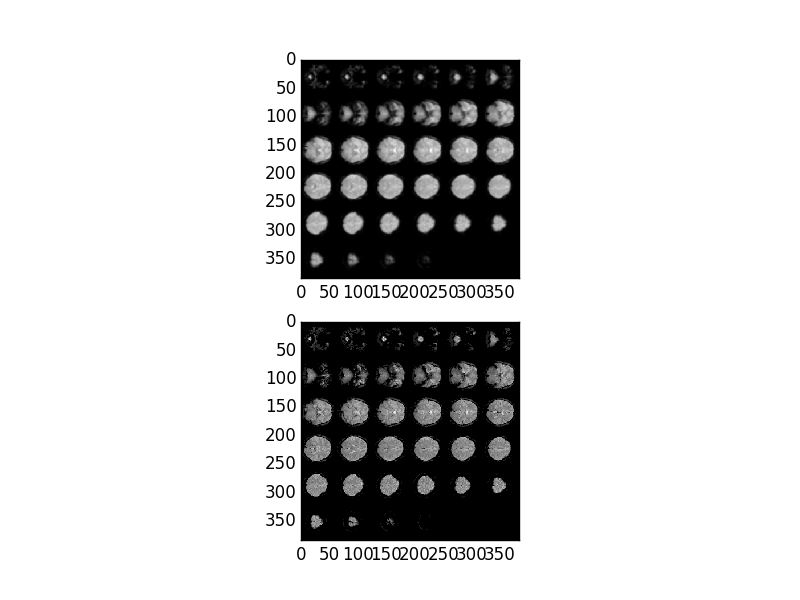
\includegraphics[scale=0.5]{images/smooth_fig.png}
\caption{Compare two bold images before and after smoothing}
\label{fig:smoothing}
\end{figure}
